\documentclass[11pt]{article}
\usepackage[utf8]{inputenc}
\usepackage[T1]{fontenc}
\usepackage[french]{babel}
\usepackage{svg}
\usepackage{listings}
\usepackage{geometry}
\usepackage{hyperref}
\usepackage{fancyhdr}
\usepackage{graphicx}
\usepackage{listings}
\usepackage{color}

\definecolor{dkgreen}{rgb}{0,0.6,0}
\definecolor{gray}{rgb}{0.5,0.5,0.5}
\definecolor{mauve}{rgb}{0.58,0,0.82}

\lstset{frame=tb,
  language=C,
  aboveskip=3mm,
  belowskip=3mm,
  showstringspaces=false,
  columns=flexible,
  numbers=left,
  basicstyle={\small\ttfamily},
  numberstyle=\tiny\color{gray},
  keywordstyle=\color{blue},
  commentstyle=\color{dkgreen},
  stringstyle=\color{mauve},
  breaklines=true,
  breakatwhitespace=true,
  tabsize=3
}

\lstset{style=mystyle}

\geometry{margin=2.5cm, vmargin=2.5cm}
\pagestyle{fancy}
\fancyhf{}

\title{Rapport Synthèse d'Image}
\author{Yann TROU et Wassim DJELLAT}
\date{Novembre 2020}

\begin{document}

\maketitle
\tableofcontents
    \vspace{\baselineskip}
    \vspace{\baselineskip}
    
    \chapter{\Large{I | Introduction}}
    \vspace{\baselineskip}
 
    \chapter{\Large{II | Création de la fourmi}} \\
    \begin{center}
        \subsection*{1. Schémas conception de la fourmi}
        \subsection*{2. Primitives}
    \end{center}
    \vspace{\baselineskip}
    
    \chapter{\Large {III | Eclairage}}
    \begin{center}
        \subsection*{1. Lumière ambiante}
        \subsection*{2. Spot}
    \end{center}
    
    \chapter{\Large {IV | Textures}}
    \begin{center}
        \subsection*{1. Textures sur les primitives}
        \subsection*{2. Matériaux}
    \end{center}
    \vspace{\baselineskip}
    
    \chapter{\Large {V | Animations}}
     \begin{center}
        \subsection*{1. Animations automatiques}
        \subsection*{2. Animations manuelles}
    \end{center}
    
    \chapter{\Large {VI| Contrôles}}
    
    
    
    
    
    
\newpage
\fancyhf{}
\lhead{I | Introduction}
\lfoot{Page \thepage}

\begin{center}
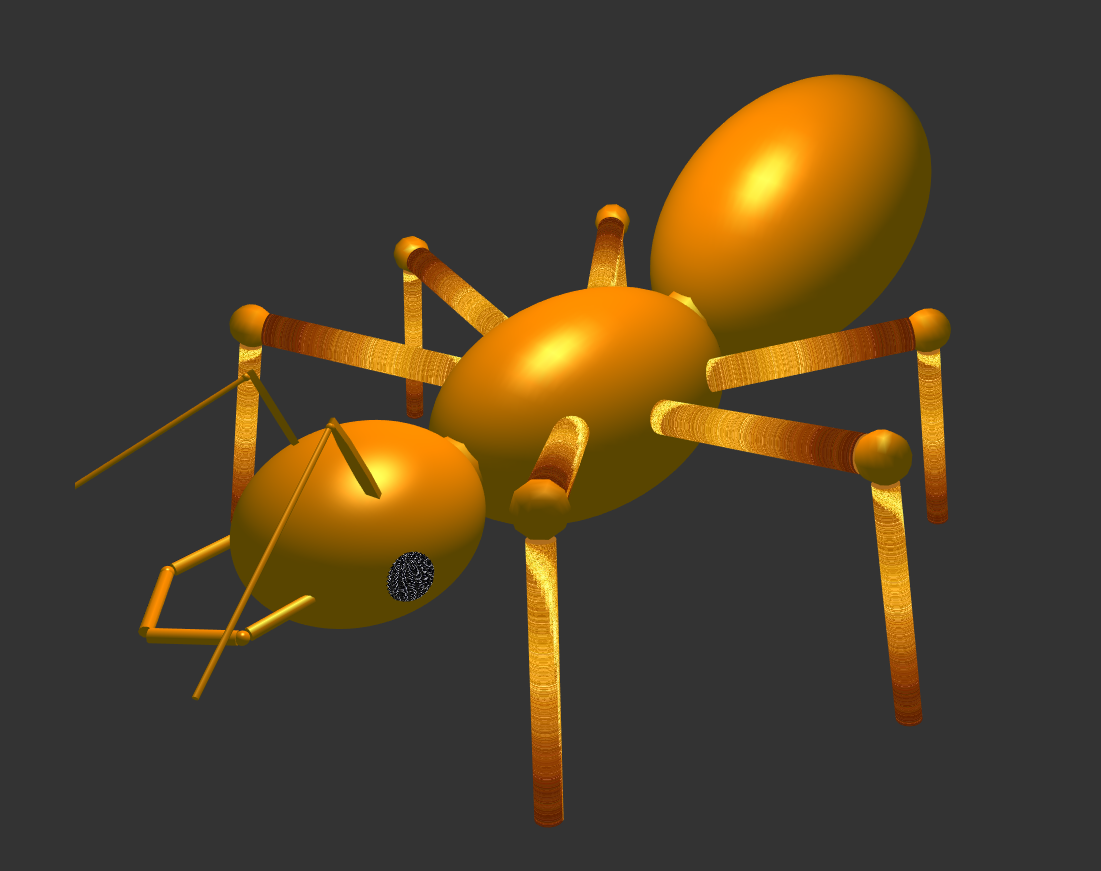
\includegraphics[scale=0.5]{photo/Capture1.PNG} 
\end{center}

\section*{Voici notre fourmi, nous avons tenté de créer une fourmi non pas réaliste mais une fourmi originale. Nous avons mis des textures dorées pour les pattes et texture d'oeil de fourmi pour les yeux. }









\newpage
\fancyhf{}
\lhead{II | Création de la fourmi}
\lfoot{Page \thepage}

\begin{center}
\includesvg[scale=0.85]{photo/FourmiS.svg}
\end{center}

R signifie Rotate / S signie Scale / T signifie Translate. \\
C'est un schémas descriptif de la conception de notre fourmi.

\subsection*{2. Primitives}

 Pour les primitives, nous avons choisi le cylindre et la sphère. Les cylindres ont ete utilisé pour creer les 6 pattes de la fourmi et biensur nous avons entouré ces pates de la texture dore.\\
 Pour les spheres, nous les avons utilisés pour former les yeux. Sur ces yeux nous avons plaqué la texture d'oeil de fourmi.



\newpage
\fancyhf{}
\lhead{III |  Eclairage}
\lfoot{Page \thepage}

    \section*{\Large{III | Eclairage}}
    \\
    Pour ce projet, il nous est demandé de gérer deux types de lumières. Nous avons donc choisi de gérer un spot et une lumiere ambiante que nous allons detailler ci-dessous.
    
    \vspace{\baselineskip}
    
    \subsection*{1. Lumière ambiante}
    \\
    La 1ere lumiere que nous avons choisi de gerer est une lumière ambiente. Elle se situera sous la fourmi et sera de couleur verte (comme si la fourmi etait sur du gazon).
    \\
    Ses paramètres sont les suivants:
    \begin{itemize}
        \item position: x=0, y=-5, z=0
        \item couleur: r=0, g=0.4, b=1.0, a=1.0
    \end{itemize}
    \\
    Ci dessous, le code représentant la lumière ambiente.
    \begin{lstlisting}
        /*Lumiere 1: ambiente verte en dessous de la fourmi*/
        posAmbient[0] = 0;
        posAmbient[1] = -5;
        posAmbient[2] = 0;
        posAmbient[3] = 0;
        GLfloat ambient2[] = { 0.0, 0.4, 0.0, 1.0 };
        glLightfv(GL_LIGHT1, GL_AMBIENT, ambient2);
        glLightfv(GL_LIGHT1, GL_POSITION, posAmbient);
        glEnable(GL_LIGHT1);
    \end{lstlisting}
    
    \vspace{\baselineskip}
    
    \subsection*{2. Spot}
    \\
    La 2e lumiere que nous utilisons est un spot de couleur blanche située au dessus de la fourmi, comme la lumière du soleil. 
    \\
    Ses parametres sont les suivants:
    \begin{itemize}
        \item position: x=0, y=5, z=0
        \item couleur (ambiente): r=0.3, g=0.3, b=0.3, a=0.3
        \item couleur (diffuse): r=1, g=1, b=1, a=1
        \item couleur (speculaire): r=1, g=1, b=1, a=1
        \item angle d'eclairage: 90 degrés
        \item attenuation lineaire: 0.1
        \item attenuation quadratique: 0.01
        \item attenuation constante: 1.0
    \end{itemize}
    Ci dessous, le code representant le spot.
    \begin{lstlisting}
        /*Lumiere 0: spot blanc au dessus de la fourmi*/
        posProj[0] = 0;
        posProj[1] = 5;
        posProj[2] = 0;
        posProj[3] = 1.0;   //important pour definir un spot
        GLfloat dirProj[] = { 0.0, 0.0, 0.0, 1.0};
        GLfloat ambient[] = { 0.3, 0.3, 0.3, 1.0 };
        GLfloat diffuse[] = { 1.0, 1.0, 1.0, 1.0 };
        GLfloat specular[] = { 1.0, 1.0, 1.0, 1.0 };
        glLightfv(GL_LIGHT0, GL_AMBIENT, ambient);
        glLightfv(GL_LIGHT0, GL_DIFFUSE, diffuse);
        glLightfv(GL_LIGHT0, GL_SPECULAR, specular);
        glLightfv(GL_LIGHT0, GL_POSITION, posProj);
        glLightfv(GL_LIGHT0, GL_SPOT_DIRECTION, dirProj);
        glLightf(GL_LIGHT0, GL_SPOT_CUTOFF, 90.0);
        glLightf(GL_LIGHT0, GL_LINEAR_ATTENUATION, 0.1);
        glLightf(GL_LIGHT0, GL_QUADRATIC_ATTENUATION, 0.01);
        glLightf(GL_LIGHT0, GL_CONSTANT_ATTENUATION, 1.0);
        glEnable(GL_LIGHT0);
    \end{lstlisting}
    
    \vspace{\baselineskip}
    
    \newpage
\fancyhf{}
\lhead{IV |  Textures}
\lfoot{Page \thepage}
    \section*{IV | Textures}
    D'apres le cahier des charges, il nous faut deux textures, une plaquee et une entouree. Nous avons donc deux textures s'appliquant sur les primitives. Aussi, comme nous utilisons des primitives de freeglut, nous avons simue les reflexions de l'or face à la lumiere.
    
    \vspace{\baselineskip}
    
    \subsection*{1. Textures sur les primitives}
    \\
    Deja comme nous avons fait le projet sur visual studio, il nous est impossible d'utiliser libjpeg pour charger des images et les utiliser. La solution que nous avons trouvé est la bibliotheque stb\_image que Yann avait vu lors de projets personnels avec openGL (c'est nous qui avons donne cette solution aux autres d'ailleurs). Cette bibliothèque tient dans un seul (gros) fichier d'en tete, et permet de charger n'importe quelle image en une simple ligne de code.
    La méthode loadJpegImage() du cours a ainsi été transformée en la méthode :
    \begin{lstlisting}
        unsigned char* loadJpegImage(const char* fichier, int* width, int* height, int* bpp)
        {
            /*chargement de l'image*/
            unsigned char* image = stbi_load(fichier, width, height, bpp, 3);
        
            /*vérification du chargement*/
            if (image == nullptr)
                std::cout << "Erreur, impossible de charger l'image " << fichier << std::endl;
            else
                std::cout << "Texture chargee: " << fichier << std::endl;
        
            return image;
        }
    \end{lstlisting}
    
    \vspace{\baselineskip}
    
    Maintenant, parlons des textures en elles-mêmes. Comme nous avons plusieurs textures, l'utilisation de glBindTexture devient obligatoire.
    \\
    Le code suivant represente le chargement et paramétrage de la texture pour la sphere (identique a celui pour charger la texture des cylindres):
    \begin{lstlisting}
        glGenTextures(1, &id_tex_sphere);
        glBindTexture(GL_TEXTURE_2D, id_tex_sphere);
        tex_sphere = loadJpegImage("noir.png", &width_tex_sphere, &height_tex_sphere, &bpp_tex_sphere);
        glTexParameteri(GL_TEXTURE_2D, GL_TEXTURE_MAG_FILTER, GL_NEAREST);
        glTexParameteri(GL_TEXTURE_2D, GL_TEXTURE_MIN_FILTER, GL_NEAREST);
        glTexImage2D(GL_TEXTURE_2D, 0, GL_RGB, width_tex_sphere, height_tex_sphere, 0, GL_RGB, GL_UNSIGNED_BYTE, tex_sphere);
        glTexEnvf(GL_TEXTURE_ENV, GL_TEXTURE_ENV_MODE, GL_REPLACE);
    \end{lstlisting}
    
    \vspace{\baselineskip}
    
    Nous avons deux textures en tout. Deja, la texture or qui est enroulee autour des cylindres des pattes suivant la formule vue en cours. Ensuite, une autre texture representant les yeux de la fourmi, plaquée sur les faces de la sphère. Comme cette texture est en trop haute resolution pour la geometrie et comme nous n'utilisons pas de mipmaps, un effet de scintillement apparait que nous avons décidé de conserver.

    \vspace{\baselineskip}
    
    \subsection*{2. Matériaux}
    \\
    Comme nous utilisons des solides de glut, leur donner un aspect ressemblant les textures nous a semble une évidence. Nous avons donc cree un materiaux ayant les réflexions de l'or à partir des valeurs vues dans le cours. 
    Le matériau a les propriétés suivantes:
    \begin{itemize}
        \item couleur(ambiante) : r=0.24725, g=0.1995, b=0.0745, a=1.0
        \item couleur (diffuse) : r=0.75164, g=0.60648, b=0.22648, a=1.0
        \item couleur (spéculaire) : r=0.628281, g=0.555802, b=0.366065, a=1.0
        \item réflexion: 51.2
    \end{itemize}
    \begin{lstlisting}
        /*application des réflections de matériau (type OR)*/
        glColorMaterial(GL_FRONT_AND_BACK, GL_AMBIENT_AND_DIFFUSE);
        GLfloat ambientOr[] = { 0.24725, 0.1995, 0.0745, 1.0f };
        GLfloat diffuseOr[] = { 0.75164, 0.60648, 0.22648, 1.0f };
        GLfloat specularOr[] = { 0.628281, 0.555802, 0.366065, 1.0f };
        GLfloat shine = 51.2;
        glMaterialfv(GL_FRONT_AND_BACK, GL_AMBIENT, ambientOr);
        glMaterialfv(GL_FRONT_AND_BACK, GL_DIFFUSE, diffuseOr);
        glMaterialfv(GL_FRONT_AND_BACK, GL_SPECULAR, specularOr);
        glMaterialf(GL_FRONT_AND_BACK, GL_SHININESS, shine);
    \end{lstlisting}
    
\newpage
\fancyhf{}
\lhead{V |  Animation}
\lfoot{Page \thepage}
    \section*{\Large{les animations}}
     \subsection*{1. Les animations automatiques}
     \\
     Les animations automatiques concernent les éléments suivants:
     \begin{itemize}
         \item Tête: mouvement de gauche à droite (de -15 degres à 15 degres)
         \item Mandibules: mouvement de l'interieur vers l'exterieur ( de -10 à 0 degres
         \item Queue: mouvement de bas en haut (de -10 à 10 degres)
         \item Antennes: mouvement de droite a gauche rapide. (de -10 à 10 degres)
     \end{itemize}
     
     \vspace{\baselineskip}
      Pour faire une animation, nous avons deux variables: la 1ere, definit le sens de l'animation. La 2e est la valeur de l'animation, generalement l'angle de la rotation.
      \\
      Le sens de l'animation est régulé avec des seuils qui sont définis dans le programme.
    
     \vspace{\baselineskip}
     
      \subsection*{2. Les animations manuelles}
      
        Pour l'animation manuelle, on a définit les fonctions suivantes pour déplacer les pattes de la fourmi:
        \begin{itemize}
            \item \[10 * cos(x * pi/2)\]
            \item \[10 * cos(x * pi/3)\]
            \item \[10 * cos(x * 2pi/3)\]
            \item \[10 * sin(x * pi/2)\]
            \item \[10 * sin(x * pi/3)\]
            \item \[10 * sin(x * 2pi/3)\]
        \end{itemize}
        Ci desssous, les formules représentées dans geogebra.
        \begin{center}
        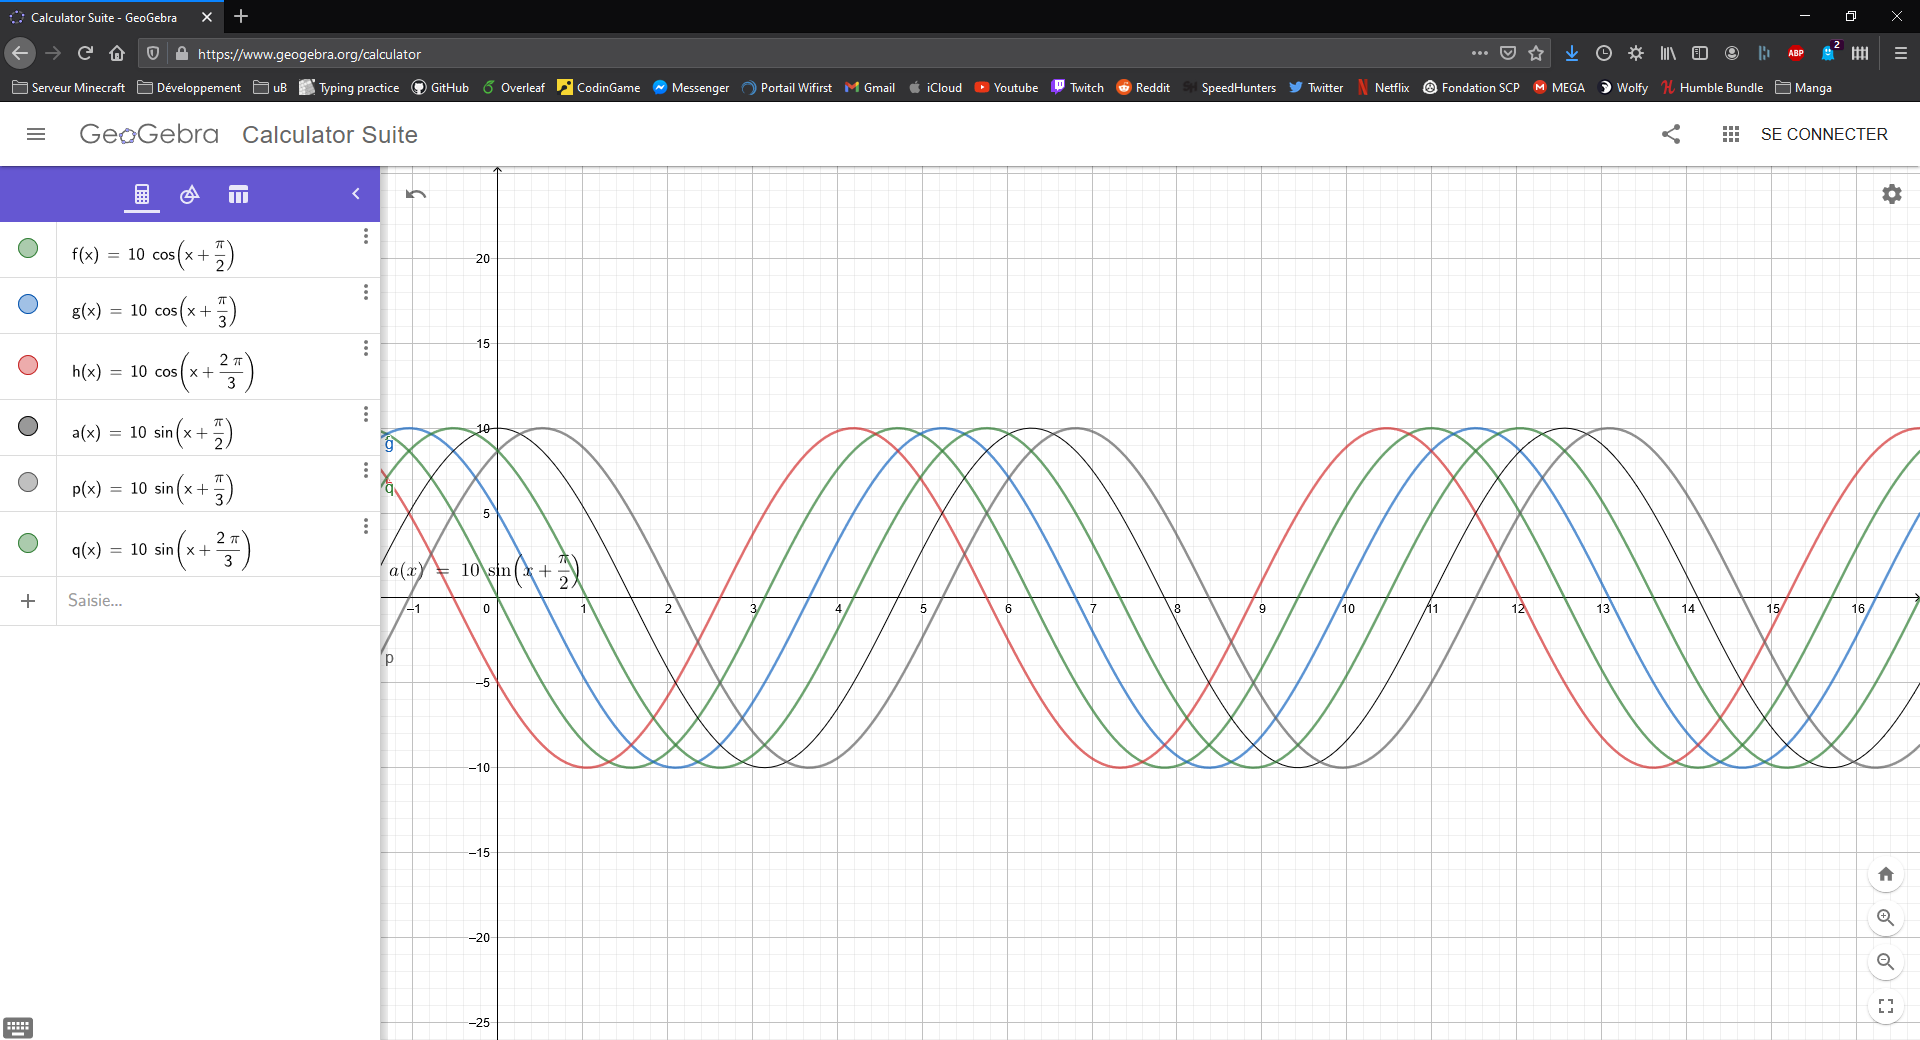
\includegraphics[scale=0.3]{photo/geogebra.PNG}
        \end{center}
        L'idée derriere l'utilisation des formules est d'avoir un mouvement fluide mais aussi que la fourmi "galope" en ayant qu'une seule patte au sol à la fois.
        L'animation manuelle est déclenchée via l'appui de la touche e, détaillé dans la rubrique controles.
\newpage
\fancyhf{}
\lhead{VI |  Controles}
\lfoot{Page \thepage}

    \section*{\Large{Les Controles}}
    
     \subsection*{1. Le Zoom}
     Ce code est pour recuperer les valeurs du Zoom applique : 
     \begin{lstlisting}
        case 'z':   /*Zoom avant*/
        zoom -= 10.0f;
        std::cout << "zoom: " << zoom << std::endl;
        glutPostRedisplay();
        break;

        case 'Z':   /*Zomm arriere*/
        zoom += 10.0f;
        std::cout << "zoom: " << zoom << std::endl;
        glutPostRedisplay();
        break;
     
     \end{lstlisting}
     
     \subsection*{2. Modification de la vue de l'objet}
     Ici nous avons la fonction qui permet de permet de modifier la vue de l'objet avec les touches :
      \begin{lstlisting}
        void specialKeyInput(int key, int x, int y)
        {
            switch (key)
            {
            case GLUT_KEY_UP:
                angley += 10.0f;
                glutPostRedisplay();
                break;
        
            case GLUT_KEY_DOWN:
                angley -= 10.0f;
                glutPostRedisplay();
                break;
        
            case GLUT_KEY_LEFT:
                anglex += 10.0f;
                glutPostRedisplay();
                break;
        
            case GLUT_KEY_RIGHT:
                anglex -= 10.0f;
                glutPostRedisplay();
                break;
            }
        }
    \end{lstlisting}
     
     
\newpage     
\subsection*{3. Touches pour animation}
Nous avons créer dans la création des pattes de la fourmi l'animation des pattes avec des formules sin et cos pour faire paraître une fourmi réel.
\begin{lstlisting}
       case 'e':
        updateAnimPattes();
        glutPostRedisplay();
        break;
\end{lstlisting}

\subsection*{4. Les affichages}

    Pour les affichages nous avons une fonction affichage() qui s'en occupe.\\
     Ce code est pour le rendu du zoom :
     \begin{lstlisting}
        /*definition de la perspective et application du zoom*/
        glMatrixMode(GL_PROJECTION);
        glLoadIdentity();
        gluPerspective(zoom, 500.0 / 500.0, 0.1, 100.0);
        glPopMatrix();
        glMatrixMode(GL_MODELVIEW);
        glLoadIdentity();
     \end{lstlisting}
     
     Ce code est pour le position de la caméra :
     \begin{lstlisting}
        /*positionnement de la camera*/
         gluLookAt(0.0, 0.0, 10.0, 0.0, 0.0, 0.0, 0.0, 1.0, 0.0);
         glRotatef(angley, 1.0, 0.0, 0.0);
         glRotatef(anglex, 0.0, 1.0, 0.0);
    \end{lstlisting}
    
    ce code est pour les formules de mouvements des pattes gauches : 
    \begin{lstlisting}
       glRotatef(10 * cos(animValue_patte + (M_PI) / 2), 1, 1, 0);
       glRotatef(10 * cos(animValue_patte + (M_PI) / 3), 1, 1, 0);
       glRotatef(10 * cos(animValue_patte + (2 * M_PI) / 3), 1, 1, 0);
    \end{lstlisting}
    
    ce code est pour les formumles de mouvements des pattes droites :
    \begin{lstlisting}
       glRotatef(10 * sin(animValue_patte + (M_PI) / 2), 1, 1, 0);
       glRotatef(10 * sin(animValue_patte + (M_PI) / 3), 1, 1, 0);
       glRotatef(10 * sin(animValue_patte + (2 * M_PI) / 3), 1, 1, 0);
    \end{lstlisting}







\end{document}
